\documentclass[11pt,a4paper]{article}
\usepackage[utf8]{inputenc}
\usepackage[margin=1in]{geometry}
\usepackage{amsmath,amssymb}
\usepackage{graphicx}
\usepackage{booktabs}
\usepackage{listings}
\usepackage{xcolor}
\usepackage{float}
\usepackage{caption}
\usepackage{hyperref}
\usepackage{pbox}
\usepackage{tikz}
\usetikzlibrary{arrows.meta,positioning,shapes.geometric}

% --- Custom Colors for Source Code Listing ---
\definecolor{mGreen}{rgb}{0,0.6,0}
\definecolor{mGray}{rgb}{0.5,0.5,0.5}
\definecolor{mPurple}{rgb}{0.58,0,0.82}
\definecolor{backgroundFix}{rgb}{0.96,0.96,0.96}

\lstdefinelanguage{NetLogo}{
    morekeywords={globals,turtles-own,patches-own,to,to-report,end,if,ifelse,
                  ask,let,set,report,repeat,stop,clear-all,reset-ticks,tick,
                  create-turtles,other,turtles,patches,in-cone,in-radius,
                  with,of,any?,count,mean,min,max,min-one-of,distance,
                  towards,atan,sin,cos,sqrt,list,item,mod,and,or,not,
                  fd,setxy,random-xcor,random-ycor,random-float,
                  patch-here,scale-color,hsb,no-turtles,myself,self,
                  black,sky,heading,shape,size,color,pcolor,xcor,ycor,
                  world-width,world-height},
    sensitive=false,
    morecomment=[l]{;},
    morestring=[b]"
}

\lstdefinestyle{NetLogoStyle}{
    backgroundcolor=\color{backgroundFix},
    commentstyle=\color{mGreen},
    keywordstyle=\color{blue}\bfseries,
    numberstyle=\tiny\color{mGray},
    stringstyle=\color{mPurple},
    basicstyle=\ttfamily\footnotesize,
    breakatwhitespace=false,
    breaklines=true,
    captionpos=b,
    keepspaces=true,
    numbers=left,
    numbersep=5pt,
    showspaces=false,
    showstringspaces=false,
    showtabs=false,
    tabsize=2,
    language=NetLogo
}

\title{
    \textbf{Laporan Tugas Besar 2 IF4021 Pemodelan dan Simulasi} \\
    \vspace{0.2cm}
    \large Pemodelan dan Simulasi Pergerakan Formasi Kawanan Burung (\textit{Boids}) Menggunakan Algoritma Craig Reynolds pada NetLogo
}

\author{
    \textbf{Brian A. Hadian} \\ 13523048 \\
    \textit{Kelompok 8}
    \makeatother
}
\date{\today}

\begin{document}

\maketitle

\hrule
\vspace{0.5cm}

% ==============================================================================
% BAGIAN 1: DESKRIPSI DAN INTERPRETASI MASALAH
% ==============================================================================
\section*{1. Deskripsi dan Interpretasi Masalah}

Fenomena pergerakan kolektif kawanan burung (\textit{flocking}) merupakan contoh klasik dari sistem kompleks adaptif (\textit{complex adaptive system}), di mana pola formasi global yang terkoordinasi muncul (\textit{emergent behavior}) dari interaksi lokal antarindividu tanpa adanya pemimpin terpusat (\textit{leaderless}). Dalam penelitian pionirnya, Craig W. Reynolds (1987, 1999) memodelkan perilaku ini melalui \textbf{algoritma Boids} (\textit{bird-oid objects}), yaitu model berbasis agen (\textit{agent-based model}) terdistribusi yang mendefinisikan gerak setiap burung melalui superposisi vektor gaya kemudi (\textit{steering forces}).

Berbeda dengan penyederhanaan model \textit{Flocking} bawaan NetLogo yang hanya memutar sudut arah secara eksklusif pada kecepatan konstan, implementasi pada tugas ini mengacu langsung pada \textbf{algoritma Boids Craig Reynolds yang sesungguhnya}: setiap agen memiliki posisi $\mathbf{p}_i \in \mathbb{R}^2$, vektor kecepatan kontinu $\mathbf{v}_i = (v_{x,i}, v_{y,i})$ yang dibatasi dalam rentang $[v_{\min}, v_{\max}]$, percepatan kemudi terbatas oleh gaya aerodinamika maksimum $F_{\max}$, serta kerucut persepsi visual (\textit{field of view}) $\theta_{\text{fov}}$ yang merepresentasikan titik buta (\textit{blind spot}) di belakang burung.

\subsection*{Karakteristik Dunia dan Persepsi Lokal Boid}
\begin{itemize}
    \item \textbf{Ruang Simulasi Toroidal:} Simulasi dijalankan pada ruang 2D kontinu berukuran $71 \times 71$ \textit{patch} ($x, y \in [-35.5, 35.5]$) dengan batas periodik (\textit{toroidal wrapping}) pada sumbu $x$ dan $y$. Perhitungan vektor perpindahan $\Delta \mathbf{p}_{ij}$ menggunakan jarak dan arah terpendek pada topologi torus.
    \item \textbf{Kerucut Persepsi (\textit{Perception Neighborhood}):} Setiap boid $i$ mengamati tetangga $j \neq i$ yang berada dalam radius persepsi $R$ dan sudut pandang depan $\theta_{\text{fov}}$ terhadap vektor kecepatannya:
    \[
        N(i) = \left\{ j \neq i \;\middle|\; \|\Delta \mathbf{p}_{ij}\| \le R \;\land\; \angle(\mathbf{v}_i, \Delta \mathbf{p}_{ij}) \le \frac{\theta_{\text{fov}}}{2} \right\}
    \]
    \item \textbf{Zona Separasi (\textit{Collision Avoidance Zone}):} Untuk mencegah tabrakan dari segala arah termasuk dari area belakang, tetangga dekat dalam radius $R_s$ didefinisikan sebagai $N_s(i) = \{ j \neq i \mid \|\Delta \mathbf{p}_{ij}\| \le R_s \}$.
\end{itemize}

\subsection*{Aturan Perilaku Kemudi (\textit{Reynolds Steering Behaviors})}
Setiap perilaku menghasilkan vektor arah tujuan $\mathbf{d}_k$, yang kemudian dikonversi menjadi gaya kemudi Reynolds dengan rumus:
\[
    \text{steer}(\mathbf{d}_k) = \operatorname{limit}\!\left( \frac{\mathbf{d}_k}{\|\mathbf{d}_k\|} v_{\max} - \mathbf{v}_i,\; F_{\max} \right)
\]
di mana $\operatorname{limit}(\mathbf{u}, M) = \mathbf{u}$ jika $\|\mathbf{u}\| \le M$, dan $\frac{M}{\|\mathbf{u}\|}\mathbf{u}$ jika $\|\mathbf{u}\| > M$. Ketiga aturan Reynolds dihitung secara simultan pada setiap langkah waktu:
\begin{enumerate}
    \item \textbf{Separation (\textit{Collision Avoidance}):} Menghindari kepadatan lokal dan tabrakan dengan tetangga di dalam $N_s(i)$ menggunakan gaya tolak berbanding terbalik kuadrat jarak:
    \[
        \mathbf{d}_{\text{sep}, i} = \frac{1}{|N_s(i)|} \sum_{j \in N_s(i)} \frac{\mathbf{p}_i - \mathbf{p}_j}{\|\mathbf{p}_i - \mathbf{p}_j\|^2} = \frac{1}{|N_s(i)|} \sum_{j \in N_s(i)} \frac{\hat{\mathbf{u}}_{ji}}{d_{ij}}, \qquad \mathbf{F}_{\text{sep}, i} = \operatorname{steer}(\mathbf{d}_{\text{sep}, i})
    \]
    \item \textbf{Alignment (\textit{Velocity Matching}):} Menyamakan vektor kecepatan dengan rata-rata kecepatan tetangga lokal pada $N(i)$:
    \[
        \mathbf{d}_{\text{align}, i} = \frac{1}{|N(i)|} \sum_{j \in N(i)} \mathbf{v}_j, \qquad \mathbf{F}_{\text{align}, i} = \operatorname{steer}(\mathbf{d}_{\text{align}, i})
    \]
    \item \textbf{Cohesion (\textit{Flock Centering}):} Mengarahkan gerak menuju pusat massa lokal dari tetangga yang terpersepsi pada $N(i)$:
    \[
        \mathbf{d}_{\text{coh}, i} = \frac{1}{|N(i)|} \sum_{j \in N(i)} \Delta \mathbf{p}_{ij}, \qquad \mathbf{F}_{\text{coh}, i} = \operatorname{steer}(\mathbf{d}_{\text{coh}, i})
    \]
    \item \textbf{Superposisi Gaya dan Integrasi Kinematika Sinkron:} Seluruh gaya dijumlahkan secara terbobot dengan bobot $(w_{\text{sep}}, w_{\text{align}}, w_{\text{coh}})$, dibatasi oleh $F_{\max}$, dan diintegrasikan secara paralel dua fase (sensing lalu update) agar bebas bias urutan agen:
    \[
        \mathbf{a}_i(t) = \operatorname{limit}\!\Big( w_{\text{sep}}\mathbf{F}_{\text{sep},i} + w_{\text{align}}\mathbf{F}_{\text{align},i} + w_{\text{coh}}\mathbf{F}_{\text{coh},i},\; F_{\max} \Big)
    \]
    \[
        \mathbf{v}_i(t+1) = \operatorname{clamp\_speed}\!\big(\mathbf{v}_i(t) + \mathbf{a}_i(t),\; v_{\min},\; v_{\max}\big), \qquad \mathbf{p}_i(t+1) = \mathbf{p}_i(t) + \mathbf{v}_i(t+1)
    \]
\end{enumerate}

\subsection*{Metrik Evaluasi Kemunculan (\textit{Emergence Metrics})}
Untuk mengukur terbentuknya formasi kawanan secara kuantitatif, simulasi mencatat metrik berikut pada setiap \textit{tick}:
\begin{itemize}
    \item \textbf{Polarisasi Global ($\Phi(t) \in [0, 1]$):} Parameter keteraturan Vicsek, $\Phi(t) = \frac{1}{N}\left\|\sum_{i=1}^{N} \frac{\mathbf{v}_i(t)}{\|\mathbf{v}_i(t)\|}\right\|$, di mana $\Phi \approx 0$ menunjukkan arah acak dan $\Phi \to 1$ menunjukkan keselarasan arah global.
    \item \textbf{Jarak Tetangga Terdekat ($\bar{d}_{\text{nn}}$ dan $d_{\min}$):} Rata-rata dan nilai minimum jarak tiap boid ke boid terdekatnya untuk memverifikasi kepatuhan terhadap zona separasi ($R_s$).
    \item \textbf{Kepadatan dan Kohesi Kawanan ($\bar{n}_{\text{nbr}}$ dan $\bar{r}_{\text{coh}}$):} Rata-rata jumlah tetangga terpersepsi per boid serta jarak rata-rata ke pusat massa lokal $\Delta \mathbf{c}_i$.
\end{itemize}

Konfigurasi parameter \textit{baseline} menggunakan $N = 150$ boid, $R = 6.0$ \textit{patch}, $R_s = 2.5$ \textit{patch}, $\theta_{\text{fov}} = 270^\circ$, bobot $(w_{\text{sep}}, w_{\text{align}}, w_{\text{coh}}) = (1.8, 1.2, 1.0)$, $v_{\min} = 0.4$, $v_{\max} = 1.0$, dan $F_{\max} = 0.10$, disimulasikan selama $400$ \textit{tick} pada NetLogo 7.0.4.

\newpage

% ==============================================================================
% BAGIAN 2: DIAGRAM SISTEM DAN TANGKAPAN LAYAR PROGRAM
% ==============================================================================
\section*{2. Diagram Sistem dan Tangkapan Layar Program}

\begin{figure}[H]
    \centering
    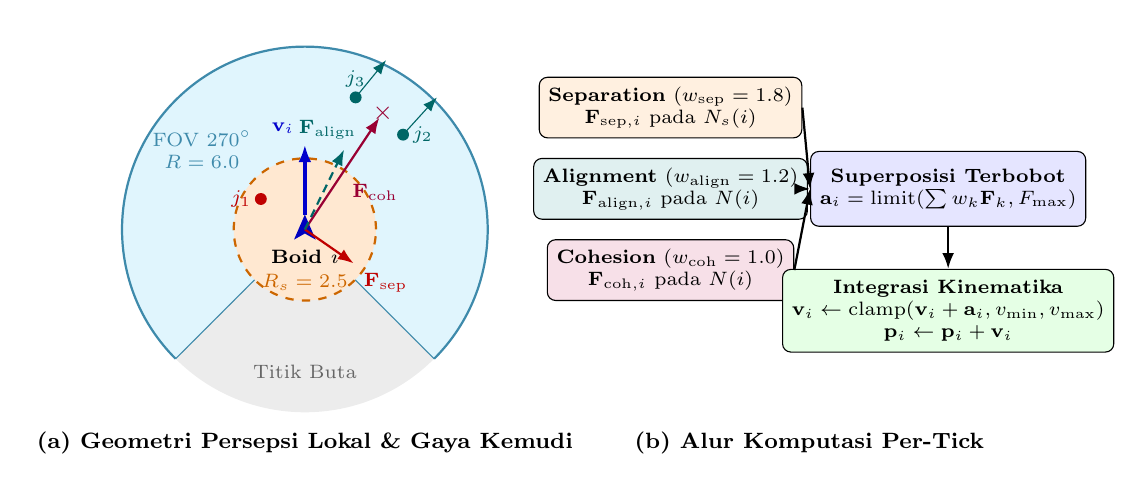
\begin{tikzpicture}[scale=0.86, every node/.style={font=\small}]
        % --- LEFT PANEL: Perception & Forces ---
        \begin{scope}[shift={(0,0)}]
            % Blind spot sector (225 to 315 deg in math coords, i.e. South)
            \fill[gray!15] (0,0) -- (225:2.7) arc (225:315:2.7) -- cycle;
            \draw[dashed, gray!70] (0,0) -- (225:2.7) (0,0) -- (315:2.7);
            % Perception cone (315 to 225+360 = 585 deg)
            \fill[cyan!12] (0,0) -- (-45:2.7) arc (-45:225:2.7) -- cycle;
            \draw[cyan!65!black, thick] (-45:2.7) arc (-45:225:2.7);
            \draw[cyan!65!black, thin] (0,0) -- (-45:2.7) (0,0) -- (225:2.7);
            % Separation circle
            \fill[orange!18] (0,0) circle (1.05);
            \draw[orange!80!black, dashed, thick] (0,0) circle (1.05);

            % Focal boid i
            \fill[blue!75!black] (0,0.22) -- (-0.16,-0.15) -- (0,-0.06) -- (0.16,-0.15) -- cycle;
            \node[below, font=\scriptsize\bfseries] at (0,-0.16) {Boid $i$};
            \draw[-{Latex[length=2.2mm]}, blue!80!black, very thick] (0,0.22) -- (0,1.25) node[above left, font=\scriptsize] {$\mathbf{v}_i$};

            % Neighbor j1 inside separation radius
            \fill[red!75!black] (-0.65,0.45) circle (2.5pt) node[left, font=\scriptsize] {$j_1$};
            \draw[-{Latex[length=2mm]}, red!75!black, thick] (0,0) -- (0.72,-0.50) node[below right, font=\scriptsize] {$\mathbf{F}_{\text{sep}}$};

            % Neighbors j2, j3 in perception cone
            \fill[teal!80!black] (1.45,1.40) circle (2.5pt) node[right, font=\scriptsize] {$j_2$};
            \draw[-{Latex[length=1.8mm]}, teal!80!black] (1.45,1.40) -- (1.95,1.95);
            \fill[teal!80!black] (0.75,1.95) circle (2.5pt) node[above, font=\scriptsize] {$j_3$};
            \draw[-{Latex[length=1.8mm]}, teal!80!black] (0.75,1.95) -- (1.20,2.50);

            % Cohesion centroid & Alignment vector
            \draw[purple!80!black, thick] (1.15,1.72) node {$\times$};
            \draw[-{Latex[length=2mm]}, purple!80!black, thick] (0,0) -- (1.10,1.65) node[midway, below right, font=\scriptsize] {$\mathbf{F}_{\text{coh}}$};
            \draw[-{Latex[length=2mm]}, teal!80!black, thick, densely dashed] (0,0) -- (0.58,1.18) node[above, font=\scriptsize, xshift=-6pt] {$\mathbf{F}_{\text{align}}$};

            % Labels
            \node[font=\scriptsize, orange!80!black] at (0,-0.78) {$R_s = 2.5$};
            \node[font=\scriptsize, cyan!65!black, align=center] at (-1.52,1.18) {FOV $270^\circ$\\$R = 6.0$};
            \node[font=\scriptsize, gray!80!black] at (0,-2.10) {Titik Buta};
            \node[font=\footnotesize\bfseries] at (0,-3.15) {(a) Geometri Persepsi Lokal \& Gaya Kemudi};
        \end{scope}

        % --- RIGHT PANEL: Steering Pipeline ---
        \begin{scope}[shift={(5.4,-2.3)}]
            \node[draw, rounded corners=3pt, fill=orange!12, minimum width=2.8cm, minimum height=0.7cm, align=center, font=\scriptsize] (sep) at (0,4.1) {\textbf{Separation} ($w_{\text{sep}}=1.8$)\\$\mathbf{F}_{\text{sep},i}$ pada $N_s(i)$};
            \node[draw, rounded corners=3pt, fill=teal!12, minimum width=2.8cm, minimum height=0.7cm, align=center, font=\scriptsize] (aln) at (0,2.9) {\textbf{Alignment} ($w_{\text{align}}=1.2$)\\$\mathbf{F}_{\text{align},i}$ pada $N(i)$};
            \node[draw, rounded corners=3pt, fill=purple!12, minimum width=2.8cm, minimum height=0.7cm, align=center, font=\scriptsize] (coh) at (0,1.7) {\textbf{Cohesion} ($w_{\text{coh}}=1.0$)\\$\mathbf{F}_{\text{coh},i}$ pada $N(i)$};

            \node[draw, rounded corners=3pt, fill=blue!10, minimum width=3.2cm, minimum height=0.95cm, align=center, font=\scriptsize] (sum) at (4.1,2.9) {\textbf{Superposisi Terbobot}\\$\mathbf{a}_i = \operatorname{limit}(\sum w_k \mathbf{F}_k, F_{\max})$};
            \node[draw, rounded corners=3pt, fill=green!10, minimum width=3.2cm, minimum height=1.05cm, align=center, font=\scriptsize] (kin) at (4.1,1.1) {\textbf{Integrasi Kinematika}\\$\mathbf{v}_i \leftarrow \operatorname{clamp}(\mathbf{v}_i+\mathbf{a}_i, v_{\min}, v_{\max})$\\$\mathbf{p}_i \leftarrow \mathbf{p}_i + \mathbf{v}_i$};

            \draw[-{Latex[length=2mm]}, thick] (sep.east) -- (sum.west);
            \draw[-{Latex[length=2mm]}, thick] (aln.east) -- (sum.west);
            \draw[-{Latex[length=2mm]}, thick] (coh.east) -- (sum.west);
            \draw[-{Latex[length=2mm]}, thick] (sum.south) -- (kin.north);
            \node[font=\footnotesize\bfseries] at (2.05,-0.85) {(b) Alur Komputasi Per-Tick};
        \end{scope}
    \end{tikzpicture}
    \caption{Diagram Arsitektur Algoritma Boids Craig Reynolds dan Pipeline Integrasi Kinematika}
    \label{fig:boids_architecture}
\end{figure}

\begin{figure}[H]
    \centering
    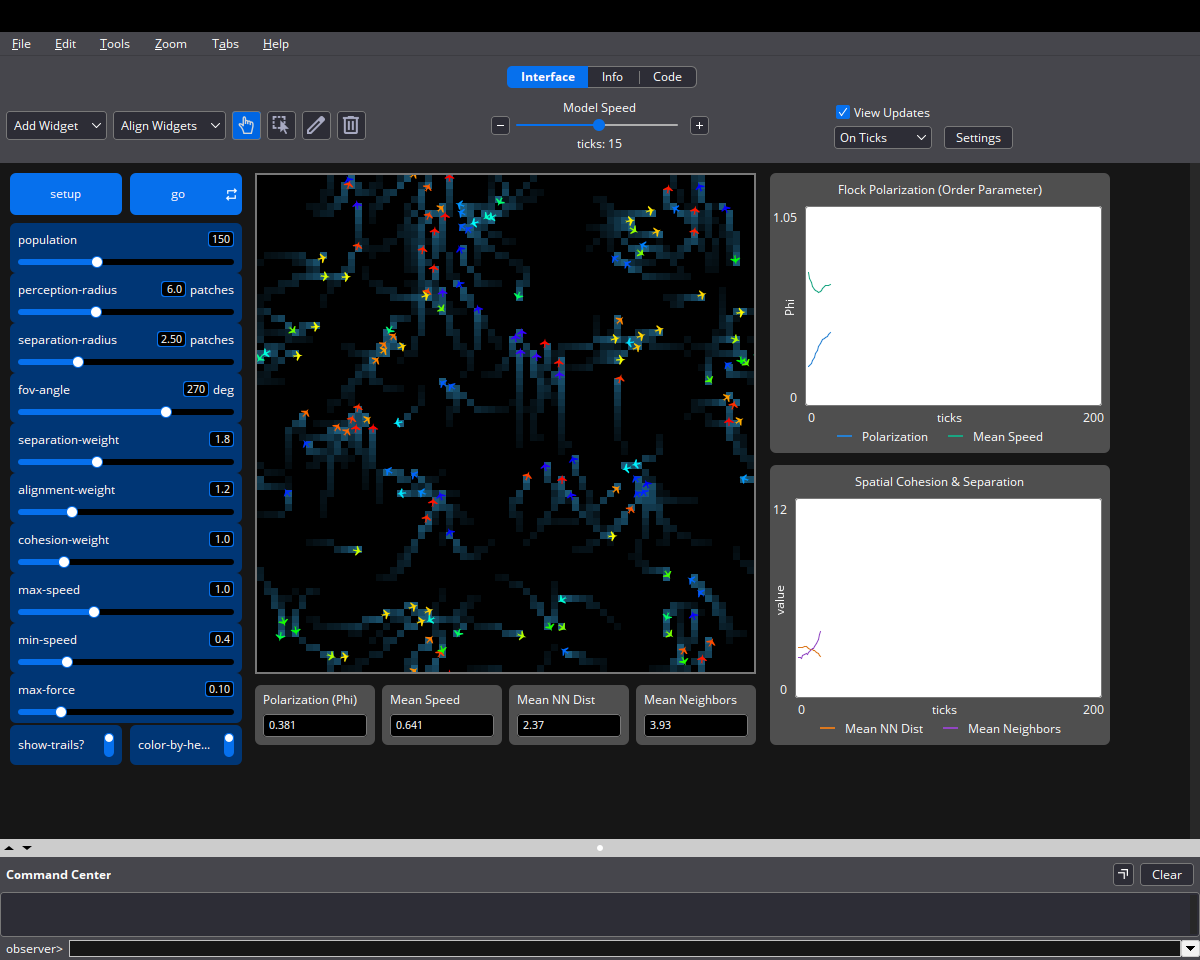
\includegraphics[width=0.84\textwidth]{netlogo_boids_early.png}
    \caption{Tangkapan Layar Aplikasi NetLogo 7.0.4 pada Fase Awal Simulasi (\texttt{ticks = 15}, $\Phi = 0.381$): Agen Masih Tersebar dan Mulai Menyelaraskan Arah Lokal}
    \label{fig:netlogo_early}
\end{figure}

\begin{figure}[H]
    \centering
    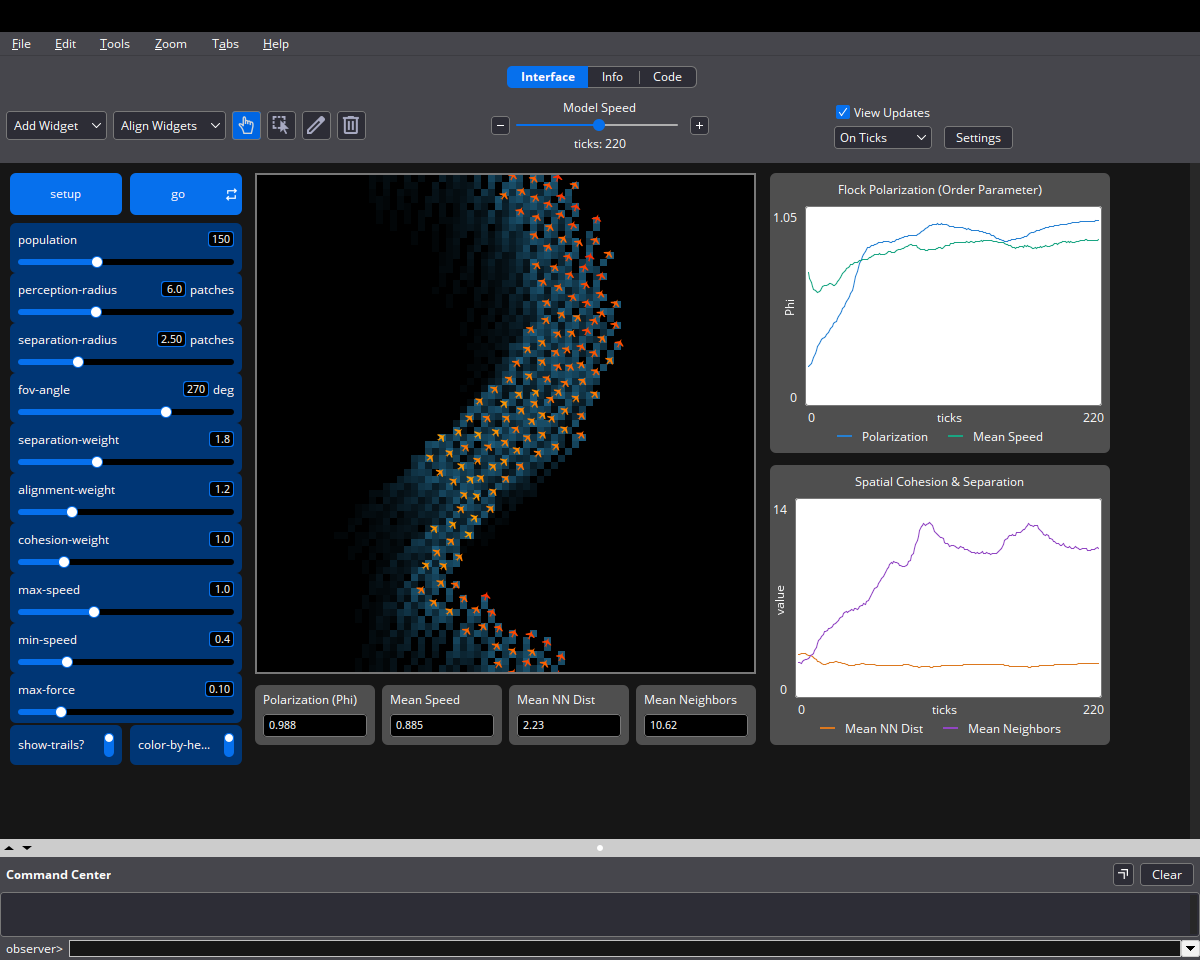
\includegraphics[width=0.84\textwidth]{netlogo_boids_sim.png}
    \caption{Tangkapan Layar Aplikasi NetLogo 7.0.4 pada Fase Konvergensi (\texttt{ticks = 220}, $\Phi = 0.988$): Formasi Kawanan Burung Terbentuk dengan Jejak Gerak Kohesif dan Grafik Polarisasi Meningkat}
    \label{fig:netlogo_converged}
\end{figure}

\begin{figure}[H]
    \centering
    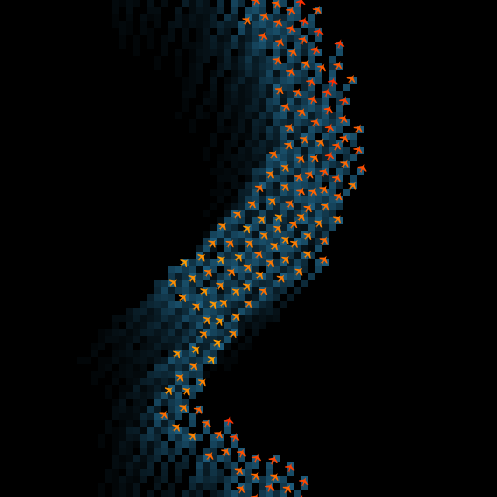
\includegraphics[width=0.52\textwidth]{netlogo_view_converged.png}
    \caption{Tampilan Detail Kanvas Simulasi Dunia Toroidal pada \texttt{ticks = 220} Menunjukkan Orientasi Formasi Burung (\textit{shape bird}) dan Jarak Separasi Antarindividu}
    \label{fig:netlogo_view_detail}
\end{figure}

\newpage

% ==============================================================================
% BAGIAN 3: KODE SUMBER PROGRAM (NETLOGO 7.0.4)
% ==============================================================================
\section*{3. Kode Sumber Program (\texttt{src/boids\_code.nlogo})}

Berikut adalah kode sumber lengkap simulasi Boids Craig Reynolds dalam bahasa pemrograman NetLogo (diekstrak dari berkas model \texttt{boids.nlogox} pada NetLogo 7.0.4).

\lstinputlisting[style=NetLogoStyle, caption={Kode Sumber Lengkap Model Simulasi Boids (\texttt{src/boids\_code.nlogo})}]{../src/boids_code.nlogo}

\newpage

% ==============================================================================
% BAGIAN 4: OUTPUT PROGRAM DAN PEMBAHASAN STATISTIK
% ==============================================================================
\section*{4. Output Program dan Pembahasan Statistik}

Pengujian kuantitatif dijalankan secara otomatis menggunakan fasilitas \textit{BehaviorSpace} pada NetLogo 7.0.4 (\texttt{netlogo-headless.sh}) melalui tiga skenario eksperimen: (a) dinamika konvergensi \textit{baseline} (5 repetisi, 400 \textit{tick}), (b) studi ablasi bobot aturan perilaku pada \texttt{ticks = 400} (5 repetisi per rezim), dan (c) analisis sensitivitas geometri persepsi $\theta_{\text{fov}} \times R$ pada \texttt{ticks = 400} (3 repetisi per kombinasi).

\subsection*{(a) Dinamika Konvergensi Simulasi \textit{Baseline} (\texttt{baseline-time-series})}
\begin{table}[H]
\centering
\small
\setlength{\tabcolsep}{5pt}
\begin{tabular}{ccccccc}
\toprule
\textbf{Tick} & \textbf{Polarisasi ($\Phi$)} & \textbf{Kecepatan ($\bar{v}$)} & \textbf{Mean NN} & \textbf{Min NN} & \textbf{Neighbors} & \textbf{Kohesi ($\bar{r}_{\text{coh}}$)} \\
\midrule
0   & $0.0723 \pm 0.0505$ & 0.698 & 2.941 & 0.208 & 2.39  & 0.000 \\
20  & $0.1414 \pm 0.1273$ & 0.648 & 2.392 & 0.431 & 4.34  & 2.478 \\
50  & $0.3563 \pm 0.2594$ & 0.757 & 2.069 & 0.350 & 9.49  & 2.377 \\
100 & $0.7908 \pm 0.1964$ & 0.827 & 2.065 & 0.768 & 11.67 & 2.222 \\
150 & $0.9429 \pm 0.0372$ & 0.862 & 2.039 & 1.044 & 12.18 & 2.083 \\
200 & $0.9877 \pm 0.0064$ & 0.859 & 2.067 & 1.153 & 12.69 & 2.068 \\
250 & $0.9719 \pm 0.0248$ & 0.874 & 2.124 & 1.203 & 11.60 & 2.053 \\
300 & $0.9721 \pm 0.0232$ & 0.864 & 2.045 & 1.101 & 12.79 & 2.037 \\
350 & $0.9869 \pm 0.0094$ & 0.866 & 2.011 & 1.051 & 13.20 & 2.017 \\
400 & $0.9912 \pm 0.0028$ & 0.861 & 1.954 & 0.997 & 13.72 & 1.945 \\
\bottomrule
\end{tabular}
\caption{Evolusi Metrik Kemunculan Boids pada Konfigurasi \textit{Baseline} (Rata-rata 5 Repetisi)}
\label{tab:baseline}
\end{table}

Pada kondisi awal (\texttt{tick = 0}), arah gerak boid terdistribusi acak dengan polarisasi rata-rata $\Phi = 0.0723$ dan jarak minimum antarindividu dapat serapat $0.208$ \textit{patch}. Memasuki \texttt{tick = 100--150}, interaksi lokal melalui aturan \textit{alignment} dan \textit{cohesion} menaikkan $\Phi$ secara tajam menjadi $0.9429$, sementara rata-rata jumlah tetangga meningkat hampir lima kali lipat dari $2.39$ menjadi $12.18$. Pada \texttt{tick = 200--400}, sistem mencapai keadaan tunak terorganisasi dengan $\Phi = 0.9912 \pm 0.0028$, jarak tetangga terdekat stabil di kisaran $\bar{d}_{\text{nn}} \approx 1.95$--$2.12$ \textit{patch}, serta $d_{\min} \approx 1.00$--$1.20$ \textit{patch} (menandakan tidak adanya tabrakan tumpang-tindih antarburung).

\subsection*{(b) Studi Ablasi Aturan Perilaku (\texttt{ablation-regimes}, \texttt{tick = 400})}
\begin{table}[H]
\centering
\small
\setlength{\tabcolsep}{4.5pt}
\begin{tabular}{lcccccc}
\toprule
\textbf{Rezim Bobot $(w_{\text{sep}}, w_{\text{align}}, w_{\text{coh}})$} & \textbf{Polarisasi ($\Phi$)} & \textbf{$\bar{v}$} & \textbf{Mean NN} & \textbf{Min NN} & \textbf{Neighbors} & \textbf{$\bar{r}_{\text{coh}}$} \\
\midrule
Full Reynolds $(1.8, 1.2, 1.0)$ & $0.9853 \pm 0.0196$ & 0.865 & 2.021 & 1.065 & 13.81 & 1.961 \\
Alignment Only $(0.0, 1.2, 0.0)$ & $0.9991 \pm 0.0019$ & 0.999 & 1.078 & 0.072 & 15.81 & 2.282 \\
Cohesion Only $(0.0, 0.0, 1.0)$ & $0.0885 \pm 0.0300$ & 0.653 & 1.772 & 0.093 & 7.06 & 2.328 \\
Separation Only $(1.8, 0.0, 0.0)$ & $0.1219 \pm 0.0582$ & 0.497 & 3.094 & 0.251 & 2.47 & 2.672 \\
Tanpa Alignment $(1.8, 0.0, 1.0)$ & $0.1143 \pm 0.0557$ & 0.567 & 2.510 & 0.458 & 3.89 & 2.339 \\
Tanpa Cohesion $(1.8, 1.2, 0.0)$ & $0.9999 \pm 0.0002$ & 1.000 & 2.888 & 2.508 & 5.76 & 2.066 \\
\bottomrule
\end{tabular}
\caption{Perbandingan Perilaku Kawanan pada Studi Ablasi (\texttt{tick = 400}, 5 Repetisi)}
\label{tab:ablation}
\end{table}

Tabel \ref{tab:ablation} membuktikan peran komplementer ketiga aturan Reynolds:
\begin{itemize}
    \item Menghilangkan \textit{separation} (\textit{Alignment Only}) menghasilkan polarisasi tinggi ($\Phi = 0.9991$), namun jarak minimum anjlok ke $d_{\min} = 0.072$ \textit{patch} karena burung saling bertumpuk pada lintasan yang sama.
    \item Menghilangkan \textit{alignment} (\textit{Cohesion Only} atau \textit{Tanpa Alignment}) menggagalkan sinkronisasi arah ($\Phi = 0.0885$--$0.1143$); burung hanya berkumpul berputar-putar secara acak di sekitar pusat massa lokal.
    \item Menghilangkan \textit{cohesion} (\textit{Tanpa Cohesion}) membuat kawanan menjadi renggang ($\bar{n}_{\text{nbr}} = 5.76$ dibanding $13.81$ pada \textit{Full Reynolds}), karena tidak ada gaya tarik jarak jauh untuk menyatukan sub-kawanan.
    \item Hanya kombinasi penuh \textbf{Full Reynolds $(1.8, 1.2, 1.0)$} yang secara simultan mencapai polarisasi tinggi ($\Phi = 0.9853$), kohesi kawanan yang rapat ($\bar{n}_{\text{nbr}} = 13.81$, $\bar{r}_{\text{coh}} = 1.961$), sekaligus keamanan jarak antarindividu ($d_{\min} = 1.065$).
\end{itemize}

\subsection*{(c) Pengaruh Geometri Persepsi: \textit{FOV} dan Radius (\texttt{fov-radius-sweep})}
\begin{table}[H]
\centering
\small
\setlength{\tabcolsep}{6pt}
\begin{tabular}{cccccc}
\toprule
\textbf{FOV $\theta_{\text{fov}}$ ($^\circ$)} & \textbf{Radius ($R$)} & \textbf{Polarisasi ($\Phi$)} & \textbf{Mean NN Dist} & \textbf{Mean Neighbors} & \textbf{Kohesi ($\bar{r}_{\text{coh}}$)} \\
\midrule
120 & 3.0 & $0.5956 \pm 0.2305$ & 2.460 & 0.84  & 1.218 \\
120 & 6.0 & $0.9743 \pm 0.0393$ & 2.183 & 5.60  & 3.520 \\
120 & 9.0 & $0.9762 \pm 0.0277$ & 2.224 & 12.50 & 5.084 \\
\midrule
180 & 3.0 & $0.9057 \pm 0.0429$ & 2.532 & 1.04  & 1.502 \\
180 & 6.0 & $0.9961 \pm 0.0014$ & 2.173 & 8.53  & 3.011 \\
180 & 9.0 & $0.9982 \pm 0.0002$ & 1.983 & 18.71 & 4.610 \\
\midrule
270 & 3.0 & $0.9273 \pm 0.0414$ & 2.527 & 1.94  & 1.423 \\
270 & 6.0 & $0.9857 \pm 0.0112$ & 2.059 & 12.49 & 1.971 \\
270 & 9.0 & $0.9931 \pm 0.0050$ & 2.160 & 22.67 & 3.172 \\
\midrule
360 & 3.0 & $0.9511 \pm 0.0009$ & 2.496 & 2.33  & 1.349 \\
360 & 6.0 & $0.9443 \pm 0.0156$ & 2.207 & 12.75 & 1.796 \\
360 & 9.0 & $0.9674 \pm 0.0313$ & 2.199 & 26.24 & 2.527 \\
\bottomrule
\end{tabular}
\caption{Analisis Sensitivitas Sudut Pandang ($\theta_{\text{fov}}$) dan Radius Persepsi ($R$) pada \texttt{tick = 400} (3 Repetisi)}
\label{tab:fov_sweep}
\end{table}

Dari Tabel \ref{tab:fov_sweep}, terlihat dua temuan penting mengenai geometri persepsi:
\begin{enumerate}
    \item \textbf{Ambang Perkolasi Interaksi:} Pada radius persepsi kecil ($R = 3.0$) dan sudut pandang sempit ($\theta_{\text{fov}} = 120^\circ$), rata-rata tetangga hanya $0.84$ sehingga aliran informasi antarburung terputus dan polarisasi hanya mencapai $\Phi = 0.5956 \pm 0.2305$. Ketika $R \ge 6.0$, jaringan interaksi lokal terhubung penuh dan $\Phi$ melonjak di atas $0.94$.
    \item \textbf{Keunggulan Titik Buta Biologis:} Untuk $R = 6.0$ dan $R = 9.0$, sudut pandang depan biologis $\theta_{\text{fov}} = 180^\circ$--$270^\circ$ menghasilkan polarisasi lebih tinggi dan lebih konsisten ($\Phi = 0.9857$--$0.9982$) dibandingkan persepsi omnidireksional $360^\circ$ ($\Phi = 0.9443$--$0.9674$). Pada $\theta_{\text{fov}} = 360^\circ$, burung di barisan depan terus-menerus tertarik ke belakang oleh gaya kohesi dari burung pengekor, memicu osilasi internal yang sedikit menurunkan keselarasan arah global.
\end{enumerate}

\section*{Referensi}
\begin{enumerate}
    \item Reynolds, C. W. (1987). \textit{Flocks, Herds, and Schools: A Distributed Behavioral Model}. Computer Graphics, 21(4), 25--34 (SIGGRAPH '87).
    \item Reynolds, C. W. (1999). \textit{Steering Behaviors For Autonomous Characters}. Proceedings of Game Developers Conference, 763--782.
    \item Vicsek, T., Czir\'ok, A., Ben-Jacob, E., Cohen, I., \& Shochet, O. (1995). \textit{Novel Type of Phase Transition in a System of Self-Driven Particles}. Physical Review Letters, 75(6), 1226--1229.
\end{enumerate}

\end{document}
